%%% template.tex
%%% This LaTeX source document can be used as the basis for your technical
%%% paper or abstract. Intentionally stripped of annotation, the parameters
%%% and commands should be adjusted for your particular paper - title, 
%%% author, article DOI, etc.
%%% The accompanying ``template.annotated.tex'' provides copious annotation
%%% for the commands and parameters found in the source document. (The code
%%% is identical in ``template.tex'' and ``template.annotated.tex.'')

\documentclass[annual]{acmsiggraph}
\TOGonlineid{45678}
\TOGvolume{0}
\TOGnumber{0}
\TOGarticleDOI{1111111.2222222}
\TOGprojectURL{}
\TOGvideoURL{}
\TOGdataURL{}
\TOGcodeURL{}
\usepackage{authblk}
\usepackage{algpseudocode}
\usepackage{algorithm}
\usepackage[T1]{fontenc}
\usepackage{hyperref}
\usepackage{graphicx}





\title{Color Correction for Optical See-Through Displays
Using Display Color Profiles}

\author[1]{Srikanth Kirshnamachari Sridharan\thanks{e-mail:kirssri@cs.umanitoba.ca}}
\author[1]{Juan David Hincapi\'{e}-Ramos\thanks{e-mail:jdhr@cs.umanitoba.ca}}
\author[2]{David Flatla \thanks{e-mail:david.flatla@usask.ca}}
\author[1]{Pourang Irani  \thanks{e-mail:irani@cs.umanitoba.ca}}

\affil[1]{Department of Computer Science, Winnipeg, Manitoba, University Of Manitoba}
\affil[2]{Department of Computer Science, Saskatoon, Saskatchewan, University Of Saskatchewan}
\renewcommand\Authands{ and }

\keywords{Color Blending, Color Correction, Optical See-through Displays, User Interface Design, Augmented Reality}

\pdfauthor{Robert A. Smith}

\begin{document}

%% \teaser{
%%   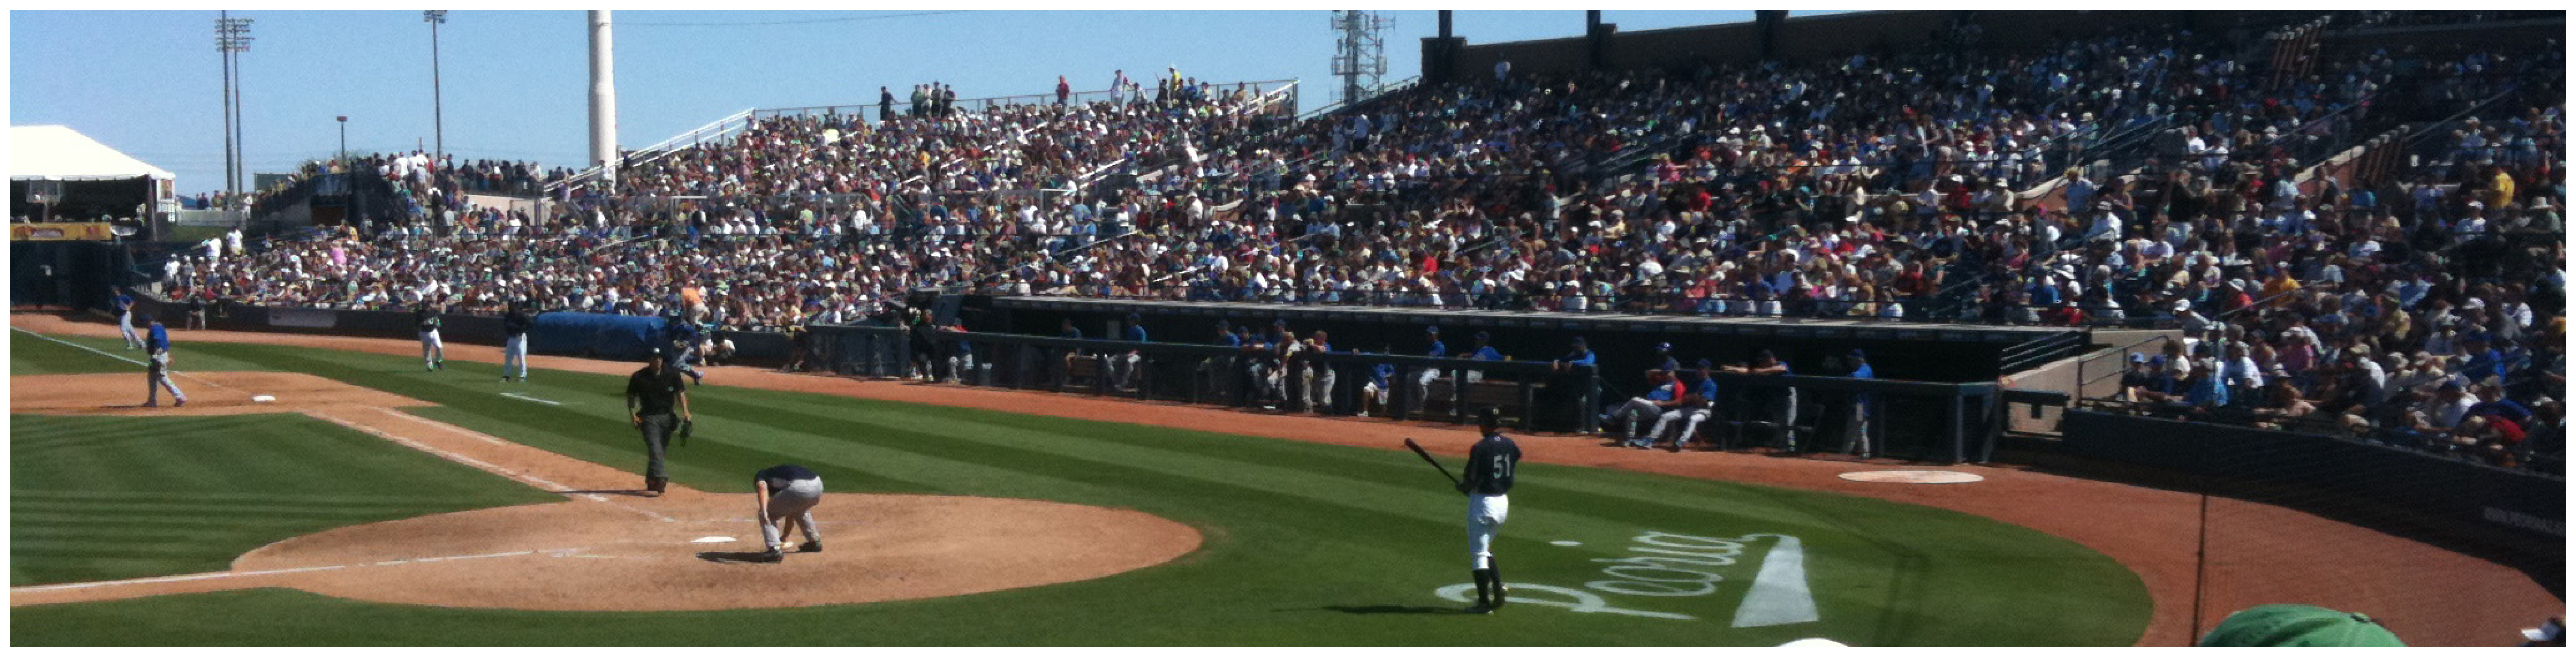
\includegraphics[height=1.5in]{images/sampleteaser}
%%   \caption{Spring Training 2009, Peoria, AZ.}
%% }

\maketitle

\begin{abstract}
In optical see-through displays, light coming from background objects mixes with the light originating from the display, causing what is known as the color blending problem. Color blending negatively affects the usability of such displays as it impacts the legibility and color encodings of digital content. Color correction aims at reducing the impact of color blending by finding an alternative display color which, once mixed with the background, results on the color originally intended.

In this paper we model color blending based on two distortions induced by the optical see-through display. The \textit{render} distortion explains how the display renders colors. The \textit{background} distortion explains how background colors are changed by the display material. We show the \textit{render} distortion has  a higher impact on color blending and propose binned-profiles (BP) - descriptors of how a display renders colors - to address it. Results show that color blending predictions using BP have a low error rate - within 9 just noticeable differences (JND) in the worst case. We introduce a color correction algorithm based on predictions using BP and measure its correction capacity. Results show light display colors can be better corrected for all backgrounds. For high intensity backgrounds light colors in the neutral and CyanBlue regions perform better. Finally, we elaborate on the applicability, design and hardware implications of our approach.
\end{abstract}

\begin{CRcatlist}
  \CRcat{H.5}{Information Interfaces and Presentation}{H.5.1}{Multimedia Information Systems - Artificial, Augmented, and Virtual Realities;} {H.5.2}{User Interfaces - Ergonomics, Evaluation / Methodology, Screen Design, Style Guides}

\end{CRcatlist}

\keywordlist

\TOGlinkslist

\copyrightspace

\section{Introduction}

Optical see-through (OST) displays allow users to view digital content and physical objects simultaneously. They come in multiple form factors (e.g. head mounted displays, projection-based and transparent LCD and OLEDs) and are widely used in augmented reality (AR) applications including medical, maintenance, education and training (see \cite{Epson2013}\cite{Lenovo2013} for a comprehensive list of applications). OST displays can be \textit{additive} (have their own light source e.g. projection-based displays or transparent OLED) or \textit{subtractive} (filter white light from an external source e.g. LCD). With a few consumer electronics starting to adopt them \cite{Lenovo2013} \cite{Epson2013}  and the continuous development of transparent OLED (Futaba Corporation \href{http://www.oled-info.com/futabas-oled-road-map-amoleds-2014-transparent-and-flexible-oleds-cars-2015}{[link]}, Fujitsu \href{http://www.fujitsu.com/be/Images/Workplace_of_the_Future.pdf} {[link]}, Winstar \href{http://www.winstar.com.tw/newspaper_ov.php?lang=en&ID=153}{[link]}) and LCD displays (Samsung NL22B \href{http://www.samsung.com/us/business/displays/digital-signage/} {[link]}, Eyevis \href{http://www.eyevis.de/index.php?article_id=163&clang=1} {[link]}) we expect they will be widely available.

An important aspect of \textit{additive} OST displays is that light coming from real-world objects mixes with the light emitted by the display: also known as color blending \cite{Gabbard:2010}. Color blending is an important issue as it affects the legibility and color-encodings of digital information and compromises the general usability of such devices. Existing solutions include using a spatial light modulator (SLM) to block background light \cite{Kiyokawa:2003}\shortcite{Kiyokawa:2002}, an approach requiring extra hardware on the display at the cost of non-transparency. Color correction is another solution where the system finds an alternative digital color which, upon blending with the background, comes closest to the desired color \cite{Weiland:2009}.

In this paper we argue that effective color correction depends on an accurate color blending model. We propose a model that takes into account two distortions induced by the display (see Figure~\ref{fig:Figure1} ): the \textit{render} and \textit{background} distortions. The \textit{render} distortion explains how a particular display renders colors. The \textit{background} distortion explains how the display material (acrylic or glass) changes background colors. Characterizing these two distortions enables us to use our model to predict color blending, which in turn allows us to create an effective color correction algorithm.

\begin{figure}[ht]
  \centering
  \includegraphics[width=3.0in]{C:/sri/acmsiggraph/images/ColorBlending.pdf}
  \caption{Color blending including the screen distortions for background and digital colors.}
  \label{fig:Figure1}
\end{figure}

In this paper we characterize the \textit{render} distortion via display binned-profiles (BP). A BP is a descriptor of how the display shows color. A BP is created by dividing the continuous universe of sRGB colors into discrete and finite bins, and measuring how the display renders each bin. We account for the \textit{background} distortion through objective measures of background colors as seen through the display material. We validate the use of BPs in our color blending model against other methods of estimating how a display renders color: the direct method (DM) and three chromatic adaptation transformation (CAT) methods. The direct method ignores that each display renders colors differently (called "trivial correction" by Weiland et al.\shortcite{Weiland:2009}). The CAT methods use known color transformation matrices based on the brightest white of the display. Our validation compares how accurately our model predicts color blending using the different methods. We used a colorimeter to objectively measure the resulting blend of different background and display colors on three optical see-through displays. Based on these measurements we computed prediction error as the difference between the predicted and the measured colors. Results showed that BP-based predictions outperform all others in our three displays.

We propose a BP-based color correction algorithm for additive displays and study it. Our results show that display colors are corrected more accurately for displays with limited color profiles and for low luminosity backgrounds. Correction is harder for high luminosity backgrounds. For the display with the largest color profile, our approach corrected light display colors better, particularly in the neutrals and CyanBlue regions.

This paper contributes to the field of optical see-though displays in several ways: 1) we introduce a color blending model for additive OST displays based on two color distortions, 2) we introduce the BP method and validate our model with it, 3) we propose BP-based color correction and studied it using a wide range of colors, and 4) we elaborate on the applicability, design and hardware implications of our approach.



\section{Background and Scope}

Color blending is the phenomenon where two colors mix to form a third. Figure~\ref{fig:Figure2}-left shows examples of color blending in an additive optical see-through display showing a yellow box over three different backgrounds: no background (black), red and blue. Figure~\ref{fig:Figure2}-right shows the corresponding shift in color\footnote{We use this 2D slice of the perceptually uniform LAB color space at D65 for presenting colors; horizontal axis maps to A and vertical axis maps to B, both ranging from -100 to 100.}: the yellow square shifts toward orange when the background is red and toward green when the background is blue. Field studies with optical see-through displays reveal that the clarity and legibility of digital colors are affected by color blending, such that the colors in text and icons are altered (change in hue) or washed out (de-saturation)\cite{Pingel:2005}. These changes affect the user interface and can render it ineffective: e.g. text might turn unreadable when washed out, or color encoded information might lose their visual meaning.

Gabbard et al.\shortcite{Gabbard:2010}, studied such color changes in optical see-through displays by building an experimental test-bed and examining display (27 colors on the edge of the RBG gamut) and background colors (6 common outdoor colors - foliage, brick, sidewalk, pavement, white and no background). Their results show that high intensity backgrounds affect all display colors by pulling them towards white, and backgrounds of different hues pull all colors toward them. Gabbard et al. \shortcite{Gabbard:2010} modeled the color blended and perceived by a user (CP) as a function of the light source (L1), the reflectance (RF) of a background object (B), the light emitted by the display (L3), the interaction of both L1 and L3 in the display (ARD), and the human perception (HP). See equation 1:
\begin{equation}
CP=HP(AD_{D}(L_{3},RF(L_{1},B)))
\end{equation}

\begin{figure}[ht]
  \centering
  \includegraphics[width=3.0in]{C:/sri/acmsiggraph/images/ColorBlendingExample.pdf}
  \caption{Examples of color blending. Left: the p3700 display shows a yellow rectangle on (1) black, (2) red and (3) blue backgrounds. Right: blend colors in LAB.}
  \label{fig:Figure2}
\end{figure}

We take this model as a starting point and un-wrap the interaction of colors on the display (ARD in equation 1) to account for two externally observable distortions: the \textit{render} and \textit{background} distortions. The \textit{render} distortion is due to the fact that each display renders digital colors differently. Figure \ref{fig:Figure3}-left shows the color red (FF0000) as rendered by different displays. Figure \ref{fig:Figure1} illustrates this distortion with the "digital color" and "color shown" circles. The \textit{background} distortion is due to the display material's effect on the background color. Figure \ref{fig:Figure3}-right shows the foliage color as seen through different displays. Figure \ref{fig:Figure1} illustrates this distortion with the "bg color" and "bg in display" circles. In our formulation we unify the light and reflectance of the background (RF(L1,B)) into the single entity "background color". We turn the interaction of light in the displays (ARD) into color addition. Moreover, we account for human perception (HP) by using the CIE XYZ and LAB color spaces which are based on human color perception. We model color blending as follows:
\begin{equation}
Blended Color=f_{render}(DC)+f_{bg}(BC)
\end{equation}

\begin{figure}[ht]
  \centering
  \includegraphics[width=3.0in]{C:/sri/acmsiggraph/images/BG_Fg_example.pdf}
  \caption{Left: \textit{Render} distortion - the color FF0000 (white border) and as displayed by three OST displays. Right: \textit{background} distortion - foliage color (white border) and as it is seen through three OST displays.}
  \label{fig:Figure3}
\end{figure}

Key to this model is the characterization of the $f_{render}$ and $f_{bg}$ distortion functions. The $f_{render}$ function describes the way a particular display shows a given digital color (DC). The $f_{bg}$ function describes the way the display material alters a background color (BC). From Figure 3 we observe that display colors change more than background colors, and therefore this paper focuses on characterizing the $f_{render}$ function. We implement this function through the binned-profile method (see section 5). Characterizing the $f_{bg}$ function requires capturing real world backgrounds \cite{Hong:2001} and creating a model of how the display material affects them (hue and luminance - see section 6 for more details). Given its complexity the $f_{bg}$ function is out of the scope of this paper and instead we used objective measures of how background colors are seen in front and through the display.


\section{Related Work}
\subsection{User, Content and Hardware Solutions}

Researchers have long discussed color blending as a significant perceptual challenge for the field of augmented reality (AR) \cite{Kruijff:2010}, especially in outdoor environments \cite{Kerr:2011}. In order to improve the display visibility users resort to strategies like looking for a dark spot (dark surface or shadow) or placing a hand in front of the display \cite{Pingel:2005}. Both strategies require users to switch context between their activity and the display which often results in missing important information. Strategies like these inspired research into ways to improve display clarity. A simple approach is to dynamically increase the intensity of the digital content (mentioned in \cite{Kiyokawa:2001}), however such solution is not always efficient \cite{Kerr:2011}. Leykin and Tuceryan \shortcite{Leykin:2004} capture the field of view of the user and classify it into zones where digital text would be readable or unreadable. In a similar fashion, Tanaka et al.\shortcite{Tanaka:2008} developed a layout system that relocates digital content to the darker areas of the display taking into account restrictions like ordering of the components.

Color blending also affects the effective occlusion of physical objects by digital content, an important issue when the real environment is enhanced with 3D virtual objects that are intended to look real, such as in architectonical previewing. Without effective occlusion, the virtual object is perceived as translucent and unreal \cite{Cakmakci:2004} and can confuse users \cite{Sekuler:1992}. Solving the occlusion problem keeps digital content from being affected by the physical objects in the background, thus solving color blending. The main approach to occlusion has been to stop the light coming from the background by enhancing head-mounted displays with spatial light modulation (SLM) devices \cite{Cakmakci:2004}\cite{Kiyokawa:2003}\shortcite{Kiyokawa:2002}\cite{Zhou:2007}. In this approach a black/white depth mask of the scene is generated with the black pixels covering the area where digital content is not to mix with the background light. Therefore, digital colors projected on the black areas are seen in their original hue and lightness. Another solution is to control the illumination of the physical objects in a way that areas behind digital content remain in the dark. Noda et al. \shortcite{Noda:1999} explored this approach by constraining physical objects to a dark room, while Bimber and Fr\H{o}lich \shortcite{Bimber:2002} implement it via occlusion shadows in a virtual showcase. Finally, occlusion can be fixed by placing parts of the optical system behind the augmented object, such as Inami et al.'s \shortcite{Inami:2000} usage of retro-reflective material as optical camouflage.

Our approach differs from these solutions as we aim not to change the location of user interface elements or to add new hardware components to the optical see-through display. Rather we seek to manipulate the color shown by the display; an approach known as colorimetric compensation or color correction.

\subsection{Color Correction Solutions}
Researchers in the field of projector-based spatial AR studied color correction as a way to enable projections on non-white and textured surfaces. Nayar et al.\shortcite{Nayar:2003} proposed a camera-based radiometric calibration model to compute the relation between the digital image and the projection on a textured surface. Their approach requires a calibration phase where known patterns are projected on the projection surface and the resulting blended images are processed to obtain compensation matrices. Bimber et al. \shortcite{Bimber:2005} extended the range of project-able color by using a transparent film and multiple projectors, taking into account the reflectance and absorption of the digital color by the projection surface. Grossberg et al. \shortcite{Grossberg:2004} extended the radiometric model to include ambient light. While these works deal primarily in the device dependent RGB space, others achieved higher correction accuracy by working on the device independent CIE XYZ color space\cite{Ashdown:2006:DSI}\cite{Menk:2011}.

Weiland et al. \shortcite{Weiland:2009} applied color correction to optical see-through displays. Their system is based on \cite{Bimber:2005} with a camera on top of the display to capture the background. Correction is achieved by subtracting the camera-captured background color from the display color. Color subtraction ignores the \textit{render} and \textit{background} distortions (similar to the direct method), and often yields colors outside the RGB space. In this paper we continue this line of work but move away from color subtraction. We focus on the actual colors a display can show and background colors as seen through the display. Our BP-based color correction uses a best-fit approach to find the display color which, upon blending, comes closest to the desired display color. Finally, we use the device independent CIE XYZ and CIE LAB color spaces, extend our study to both projector-based and T-OLED (Transparent Organic Light Emitting Diode) displays, and present results quantitatively.

\section{Experimental Test-Bed}

Figure \ref{fig:Figure4} show our experimental test-bed built (1) to generate various background colors, (2) to show display colors on multiple optical see-through displays, and (3) to measure color blending.
\begin{figure}[ht]
  \centering
  \includegraphics[width=3.0in,height=2.5in]{C:/sri/acmsiggraph/images/setup.pdf}
  \caption{Experimental test-bed, Top: Component diagram. Bottom-Left: Actual set-up with a projector display. Bottom-Right: T-OLED display.}
  \label{fig:Figure4}
\end{figure}

To generate different backgrounds we use a Dell U2312HM VGA LCD display calibrated at the standard D65 white point, the standard outdoors lighting condition. This approach to generating background colors is limited by the color gamut of the LCD. Our test-bed differs from previous systems \cite{Gabbard:2010} which prioritize the capacity to obtain background colors as seen in nature. Our design prioritizes the capacity to automatically produce a wide variety of background colors. For our experiments we used background colors from the ColorChecker Color Rendition Chart \shortcite{McCamy:1976} because they mimic colors of everyday natural objects like skin, foliage and flowers. Figure \ref{fig:Figure6}A shows the difference between theoretical background colors and how our test-bed produces them.
\begin{figure*}[ht]
  \centering
  \includegraphics[width=\textwidth]{C:/sri/acmsiggraph/images/lab_profile.pdf}
  \caption{(A) sRGB gamut on the LAB color space, (B) the binned gamut, and the binned profile for the (C) p3700 and (D) p2200 projector-based displays, and for (E) for the T-OLED display.}
  \label{fig:Figure5}
  \end{figure*}

Our test-bed works with three optical see-through displays: two projector-based and one transparent OLED. The projector-based displays use a 3 mm transparent acrylic surface covered with a Lumisty MFY 2555 film and one of the two projectors at $40^\circ$. The first projector is an Epson 1705 with 2200 lumens, hereafter called the p2200 display. The second projector is an Epson VS35ow with 3700 lumens, hereafter called the p3700 display. For the transparent OLED display we used a Lenovo S800 phone\shortcite{Lenovo2013} which has a 240x320 transparent OLED display at 167 ppi, hereafter called the T-OLED display. The T-OLED display is covered in acrylic and is 9 mm thick. The test-bed holds the displays at 20 cm in front of the background LCD.
\begin{table}[ht]
\caption{White points for all three displays.} % title of Table
\centering % used for centering table
\begin{tabular}{c c c c c} % centered columns (4 columns)
\hline\hline %inserts double horizontal lines
 &  & p2200 & p3700 & T-OLED \\  % inserts table 
%heading
\hline\hline\\  % inserts single horizontal line
	   & X & 0.2655720 & 0.9504 & 0.383264\\ % inserting body of the table
No BG  & Y & 0.282182 & 1 & 0.395001\\
	   & Z & 0.481033 & 1.0888 & 0.369982\\ [0.5ex]
\hline\\  %inserts single line
		 & X & 0.9504 & 0.9504 & 0.724775\\
White BG & Y & 0.990041 & 1 & 0.759896\\
		 & Z & 1.0888 & 1.0888 & 0.727336\\ [0.5ex] % [1ex] adds vertical space
\hline %inserts single line
\end{tabular}
\label{table:1} % is used to refer this table in the text
\end{table}

To examine background and display colors and the resulting color blends we used the notations of the Commision Internationale de l'\'{E}clairage (CIE) color model. We use the CIE 1931 XYZ color space for color measurement and addition required by our model. The XYZ color space resembles the working of the human visual system which is more sensitive to greens and therefore not a perceptually uniform color space. We used the CIE 1976 LAB color space, a perceptually uniform color space, to calculate the perceptual difference between colors; e.g. the distance between a color and its shift when blended, or the distance between a prediction and the measured blend.


To collect data we used a Konica Minolta CS-200 luminance and color meter at 0.2 degrees (standard observer angle). The colorimeter measures colors in the XYZ color space. In order to convert these values into normalized LAB we use the measured white point of the displays involved as explained by Gabbard et al. \shortcite{Gabbard:2010}. For both p2200 and p3700 displays we measured the XYZ white points of the Lumisty surface at 5 different points: one near the each of the display's four corners and one in the center. For both projectors all measurements of the white point remained the same. We located the colorimeter at 20 cm away from the see-through display and pointing at the center. After calibrating the background LCD to D65 (measured at 0.9504, 1, 1.0888) we measured the following two combinations of the white point per display and recorded the average of 100 measures per combination(see Table 1):

1. See-through showing white and bg LCD turned off.\\
2. Both see-through and bg LCD showing white.

The displays and the colorimeter were connected to the same controlling computer and were kept away from the ambient light by a light enclosure (represented in Figure \ref{fig:Figure4} as the dark cave).

\section{The Binned Profile Method}

In order to build a reliable color correction system, it is necessary to have an accurate model of color blending. Equation 2 explains our model and this section presents a method to implement the $f_{render}$ distortion function. This function receives the color the display wants to show as a parameter and return the color the display actually shows.

We propose binned-profiles (BP), a method which divides the sRGB color space (over 16 million colors) into a smaller set of 8376 perceptually different bins. To create the bins we translate the sRGB gamut into the CIE LAB color space and divided it into bins of 5x5x5 - an approach proposed by Heer and Stone \shortcite{Heer:2012}. This approach guaranties all colors inside a bin are within one Just Noticeable Difference (1 JND, approx. 2.3 in Euclidean distance), such that they are perceived as the same color by a human observer \cite{Mahy:1994}. Figure \ref{fig:Figure5}A-B shows the sRGB gamut on the CIE LAB color space and the binned result. Then, we measured how each bin is rendered by each of our three displays(8376 colors) on a black background. Each color was captured using the colorimeter in XYZ and we transferred it into the CIE LAB color space using the reference white points given in Table 1(top row). Based on these measurements we created a color profile for each display. Figure \ref{fig:Figure5}C-E presents the display profiles, with the p3700 almost matching color capacity of sRGB(C), and considerable reductions of color capacity for the p2200(D) and T-OLED displays(E).

\begin{algorithm}
\caption{Binned-Profile based prediction algorithm}
\begin{algorithmic}
	 \label{alg:1}
	\Procedure{BP-Prediction   }{$Display$,$Foreground$,\ $Background$}
	\State $BinForeground=findBin(Foreground)$
    \State $DispForeground$=$lookup$($Display$,$BinForeground)$
	\State $Prediction$=$addXYZ$($DispForeground$,$Background)$
	\textbf{return}$Prediction$
	\EndProcedure
  \end{algorithmic}
\end{algorithm}

\begin{figure*}[ht]
  \centering
  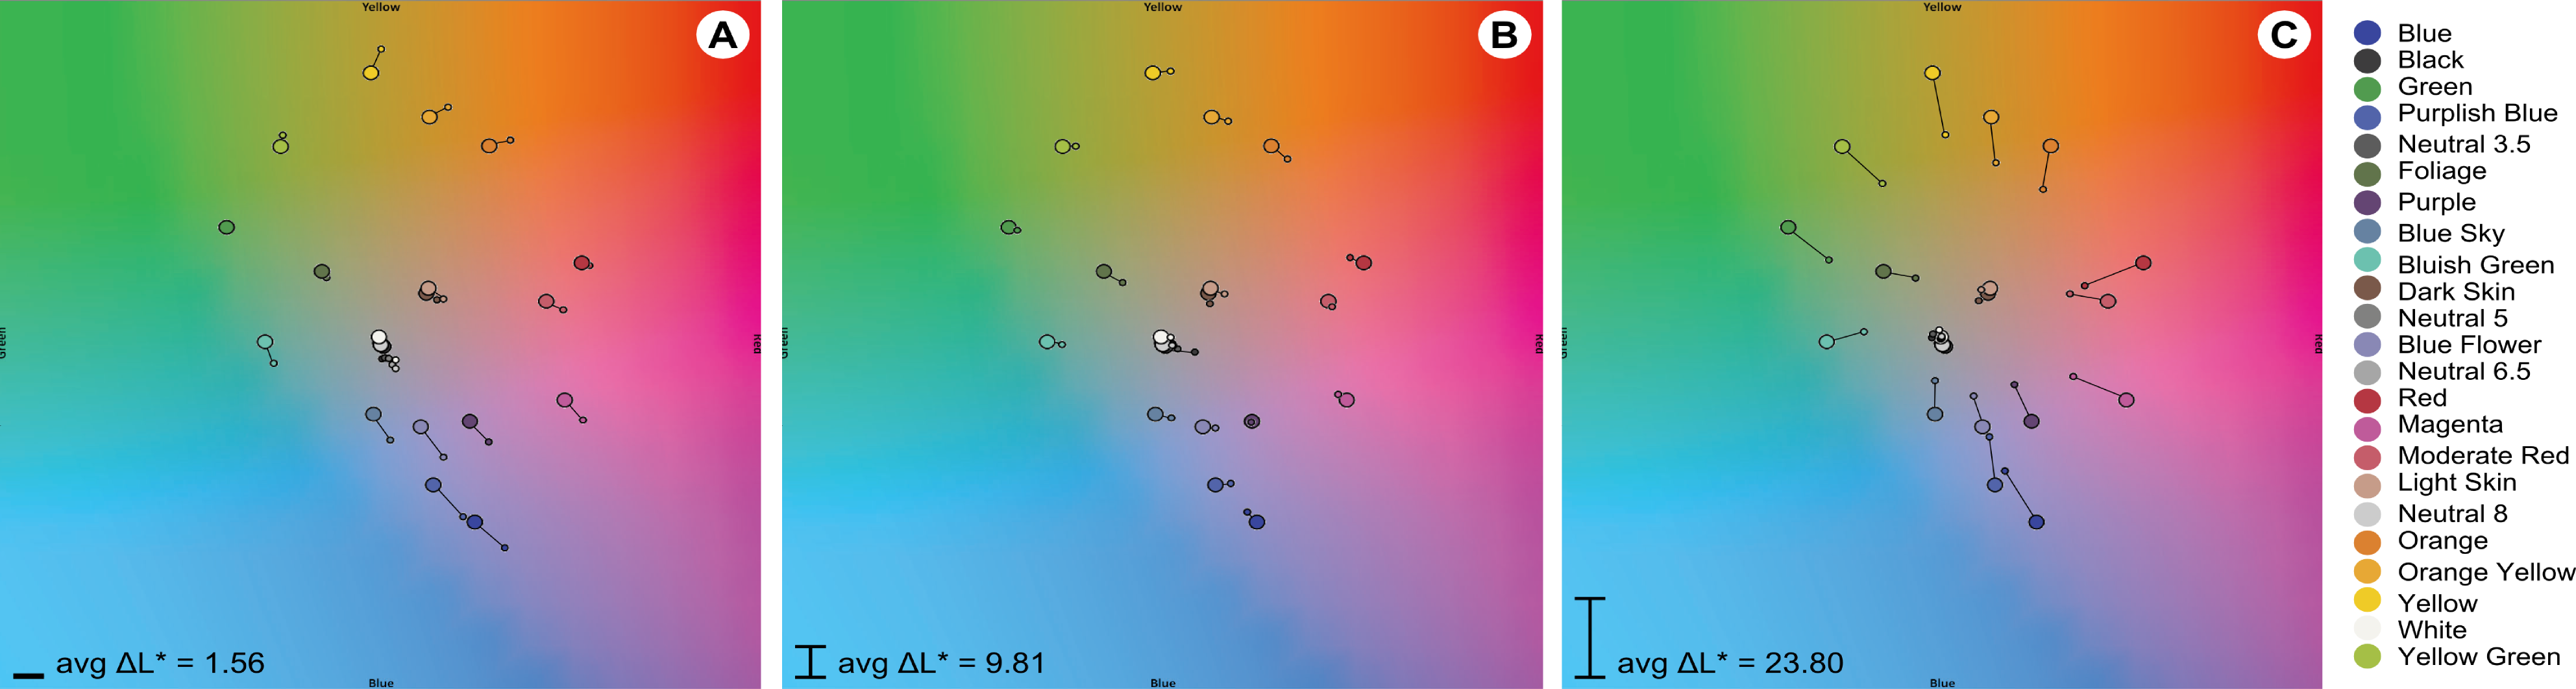
\includegraphics[width=\textwidth,height =1.6in]{C:/sri/acmsiggraph/images/bg.pdf}
  \caption{ColorChecker bg colors as (A) shown by the background LCD, (B) as seen through the p2200 and p3700 displays, and (C) as seen through the T-OLED display. Bigger circles = original color. Small circle = measured color.}
  \label{fig:Figure6}
\end{figure*}

Color blending prediction based on the BP method consists of using the display profile as a lookup table (see Algorithm 1). To find out how a display represents a digital color we first translate the color to its closest bin in LAB space and use it as a key in the profile lookup table. The color associated with the key is the one the display actually shows (Color Shown in Figure \ref{fig:Figure1}). We use this color in our color blending model (equation 2): we add it to the background in CIE XYZ and obtain the color blend.

\subsection{Binned-Profile Validation}
In order to assess the validity of BP method in our color blending model, we measure the error of the prediction and compare it to the predictions using the direct method (DM) and three chromatic adaptation transformation (CAT) methods. Error is measured as the difference between the predicted and the measured color blend (computed in CIE LAB). When using the direct method the digital color is simply added to the background. CAT are established methods to estimate the colors a display can render based on the brightest white it can emit. In other words, CAT could potentially account for the  $f_{render}$ distortion function. CAT is based on matrices and researchers have proposed CAT methods which rely on different matrices. When using the CAT methods we transformed the display color using the respective CAT matrix before adding it to the background. We chose three popular CAT methods: Bradford,Von Kries \cite{Susstrunk:2000}, and XYZ Scaling \cite{CAT2013}. We selected those methods due to their popularity in the literature.

As discussed before, measuring the background color and characterizing the effect of the \textit{background} distortion ($f_{bg}$ function) is out of the scope of this paper. We work under the assumption that such color is available at a per-pixel level. However, to explore the impact of the \textit{background} distortion, we compare two possible background detection implementations: \textit{plain} and \textit{adjusted}. The background color is \textit{plain} if the system ignores the effect of the distortion and feeds it to the model as it is measured, so that $f_{bg}$(background)=background. The background color is \textit{adjusted} if the system accounts for the \textit{background} distortion and transforms it before feeding it to the model (see Bg in Display,Figure \ref{fig:Figure1}).

We considered 23 colors of the ColorChecker Color Rendition Chart \shortcite{McCamy:1976} at D65, a representative set of naturally occurring colors (the 24th ColorChecker color is outside of the sRGB gamut). We measured the colors as shown by the background LCD. These values correspond to the \textit{plain} background configuration(see Figure \ref{fig:Figure6}A). We also measured how each background color would be seen through the see-through displays (see Figure \ref{fig:Figure6}B-C). These values correspond to the \textit{adjusted}  background configuration for each display. The measured \textit{adjusted} values show displacement in 'a' and 'b', but also a considerable reduction of L; this is due to the display material absorbing some of the light from the background (the \textit{background} distortion). It is to be noted that there was a significant impact of the T-OLED display on all axes of the background color.

\subsection{Data Collection}
We used the 23 ColorChecker backgrounds against 838 random display colors (10\% of the size of the bin). We measured the resulting blend of each pair for each of our three displays capturing a total of 23x838 = 19,274 measurements per display and 19,274x3 = 57,822 measurements in total. We converted the blending measurements into CIE LAB using the white points from Table 1. We predicted the resulting color blend for each combination of display color method (5 methods), background configuration (2 configurations) and display (3 displays). We obtained 5x2 = 10 predictions per blending, 5x2x23x838 = 192,740 predictions per display, for a total of 192,740x3 = 570,822. We computed the prediction error by calculating the Euclidean distance in CIE LAB color space between each prediction and the actual measurement.

\begin{table}[ht]
\caption{Kruskal-Wallis test for prediction error.} % title of Table
\centering % used for centering table
\begin{tabular}{c c c c c c} % centered columns (4 columns)
\hline
\hline
 Display & Method & Bg-Type & df & $\chi^2$ & Sig \\   % inserts table 
%heading
\hline\hline  % inserts single horizontal line
X&--&--&2&32152&<0.001\\
--&X&--&1&698210&< 0.001\\
--&--&X&1&25745&< 0.001\\
--&X&X&3&104717&< 0.001\\
X&X&--&5&101643&< 0.001\\
X&--&X&5&60583&< 0.001\\
X&X&X&11&142259&< 0.001\\
\hline %inserts single line
&&Post&Hoc&\\
\hline
--&Both&Adjusted&1&59437&< 0.001\\
--&Both&Plain&1&21613&< 0.001\\
--&BP&Both&1&52494&< 0.001\\
--&DM&Both&1&2157&< 0.001\\
\hline
\end{tabular}
\label{table:2} % is used to refer this table in the text
\end{table}

\subsection{Results}
Figure \ref{fig:Figure7} summarizes the results for our prediction study using vertical histograms. Each histogram represents the prediction error of all display colors for a given background: lower error (zero difference in LAB) is the bottom of the graph and color saturation represents the height of the histogram. A visual inspection of the results shows that for all conditions the CAT-based predictions performed worst, with a high spread in error and an average far from optimal (in the case of the p3700 display, all CAT-based predictions perform the same because the white point of this display is exactly D65). Thus we exclude the CAT methods from the rest of this analysis. Results did not have a normal distribution and therefore we used the Kruskal-Wallis H test for non-parametric data. Table 2 shows the results of our analysis. Results showed a main effect of \textit{display, method} and \textit{background} configuration. There were also significant interaction effects between all independent variables.

\begin{figure*}[ht]
  \centering
  \includegraphics[width=\textwidth , height=2.5in]{C:/sri/acmsiggraph/images/predictionResults.pdf}
  \caption{Prediction results of p2200, p3700 and T-OLED displays, with 5 prediction methods, in \textit{plain}  and \textit{adjusted}  bg configurations.}
  \label{fig:Figure7}
\end{figure*}

For the p2200 display BP-based prediction performed best in each background configuration (\textit{plain} : 10.01 - \textit{adjusted} : 4.98). DM-based prediction presented only a small difference between background configurations (\textit{plain} : 22.71 - \textit{adjusted} : 22.06). We observe a similar pattern for the p3700 display where BP-based prediction has lower error for both background configurations (\textit{plain} : 10.28 - \textit{adjusted} : 2.77) than the DM-based prediction (\textit{plain} : 17.5 - \textit{adjusted} : 13.67). Finally, when applied to the T-OLED display BP-based prediction also performed better (\textit{plain} :25.63 - \textit{adjusted} : 8.24) than DM-based prediction (\textit{plain} : 34.37 - \textit{adjusted} : 32.26).
\begin{figure}[ht]
  \centering
  \includegraphics[width=3in,height=1.3in]{C:/sri/acmsiggraph/images/KW_PResults.pdf}
  \caption{Prediction error for the three displays, with the BP and DM , for two background configurations.}
  \label{fig:Figure8}
\end{figure}

Overall, Figure \ref{fig:Figure8} shows that BP-based predictions outperform all other methods we tested across the 23 backgrounds. Moreover, this lower error rate exists for both the \textit{plain}  and \textit{adjusted}  background configurations. Our results confirm the importance of the \textit{render} distortion (how the display represents digital color) as the dominant factor for color blending. More importantly, our results highlight the limitations of the direct method (ignoring the display distortion) and the inadequacy of any of the three CAT methods we tested. Finally, results show that considering the \textit{background} distortion decreases prediction error, reducing the error by more than half in all displays when using the BP method. For the p3700 display prediction error using the BP method with the \textit{adjusted}  background was 2.77 or about 1 JND.

\section{Color correction}
Color correction aims at finding an alternative color which, upon mixing with the background, results with the color originally desired by the designer. In this section we propose a color correction approach for optical see-through displays based on the BP method. When correcting a color for a given background, the system predicts how each color of that particular display's profile blends with the background. Then the system finds the prediction which comes closest to the originally intended color - a best fit approach. This algorithm is described in Algorithm 2: First, the display color (Foreground - the sRGB color the system wants to paint on the screen) is mapped to the closest of the bin (BinForeground - see Figure \ref{fig:Figure5}B) with respect to the display type(Display). Second, based on the display profile, the bin color is mapped to its actual representation (DispForeground - the way such bin is actually shown by the display). Third, for each bin on the display profile, the system predicts how it blends with the background (Prediction) and calculates the distance between the prediction and the display color (TmpError). The system selects the prediction with the lowest distance (ColorToShow) and converts it to the corresponding binned color that produces it via a reverse lookup (CorrectedColor). Finally the display shows the corrected color.
\begin{algorithm}
\caption{Binned-Profile color correction algorithm.}
\begin{algorithmic}
\Procedure{BP-Preservation  }{$Display$,$Foreground$,\ $Background$}
	\State $BinForeground=findBin(Foreground)$
    \State $DispForeground=lookup(Display,BinForeground)$
    \State $Error=INFINITY$
	\State \textbf{for each} $Color$ \textbf{in} $Display$
     \State \quad$Prediction=addXYZ(Color,Background)$
     \State \quad$TmpError$=$distance$($Prediction$,$DispForeground)$
	 \State \quad\textbf{if} $TmpError$\textbf{<}$ Error$
	  \State \qquad $Error=TmpError$
	  \State \qquad$ColorToShow=Color$
   	 \State $CorrectedColor$=$revLookup$($Display$,$ColorToShow)$
   	\State \textbf{end for}
	\State \textbf{return}$CorrectedColor$
	\EndProcedure
  \end{algorithmic}
\label{alg:2}
\end{algorithm}
It's important to note that our algorithm aims at correcting the color the display actually shows, rather than the application defined foreground. Moreover, our algorithm avoids using color subtraction (CorrectedColor=foreground-background) for two reasons: first, similarly to the direct model for color prediction, color subtraction ignores the display profile leading to an incorrect target for correction. Second, because color subtraction often results in values which are outside the display profile.

\subsection{Data Collection}
The goal of this study is to explore how well the BP-based correction algorithm performs for different common backgrounds. We applied BP-based color correction on the p3700, p2200 and T-OLED see-through displays for the 23 ColorCheck \textit{adjusted}  backgrounds. We selected 200 random display colors for each background, corrected them, and measured resulting color blend amounting to 23x200 = 4600 measures per display. We collected a total of 23x200x3=13800 measurements for all three displays. We then calculate correction error as the difference between the measured blend and the intended display color.
\begin{figure}[ht]
  \centering
  \includegraphics[width=3in,height=1.2in]{C:/sri/acmsiggraph/images/ColorReg.pdf}
  \caption{Display color groups. Left: neutral colors within 10 JNDs from the L axis. Right: 6 chromatic regions - YellowGreen, GreenCyan, CyanBlue, BlueMagenta, MagentaRed and RedYellow.}
\label{fig:Figure9}
\end{figure}


We took a two-step approach to analyzing the collected data. In the first step we looked at the general correction capacity of the algorithm for the three displays. In the second step we focused on the p3700 display as it can reproduce a wider variety of colors (see Figure \ref{fig:Figure5}C-E for the color profile of each display). For this display we grouped the display colors into 10 groups: dark colors (L < 50), light colors (L >= 50), dark and light neutrals (neutrals are located within 10 JNDs of the L axis), and 6 chromatic regions according to the color circle. Figure \ref{fig:Figure9} shows (left) the dark and light neutrals, and (right) the 6 chromatic regions. Note that each display color might belong to more than one group. Similarly, we divided the ColorCheck backgrounds into high intensity colors (L >= 50) resembling daylight conditions like white and yellows, and low intensity colors (L < 50) resembling night conditions like black and blue. Figure \ref{fig:Figure10} shows the background color groups.

\begin{figure}[ht]
  \centering
  \includegraphics[width=2.7in,height=0.7in]{C:/sri/acmsiggraph/images/ColorName.pdf}
  \caption{Low and High intensity background groups.}
  \label{fig:Figure10}
\end{figure}

\subsection{Results}
For analyzing the correction results we used vertical histograms together with color heat-maps (see Figure \ref{fig:Figure11}-Top-Right). The color heat-map reveals how well our algorithm corrects regions of the LAB color space for a given set of background colors. The color heat-map divides the LAB D65 slice into a 30x30 grid. Each grid cell is colored in blue (0000FF) with the opacity moving from 0 to 1, where the opacity is relative to the average correction error (ranging from 0 to 100+) of all colors in that cell. If the sample did not contain corrections for display colors in a given cell, the cell has no blue box. If the sample contains corrections for a given cell, the error of each correction is calculated and averaged with the rest. Cells in which colors are well corrected (lower correction error) in average result in a faint blue. Cells in which colors cannot be corrected in average (higher correction error) result in a dark blue. Figure \ref{fig:Figure11} shows the general correction results for all background and display colors on the three displays.
\begin{figure}[ht]
  \centering
  \includegraphics[width=3.0in,height=2.5in]{C:/sri/acmsiggraph/images/CorrectionResult.pdf}
  \caption{Overview of correction error rate. Heatmap - darker blue indicates higher correction error.}
  \label{fig:Figure11}
\end{figure}

A visual inspection of the results reveals that correction works better for low luminosity backgrounds (toward the left of the vertical histogram) for all three displays. Results also show corrections have lower error for the p2200 and T-OLED displays (fainter blue boxes in the heat-map and more concentrated vertical histograms). This could be explained by the limited range of colors these displays render (concentrated in a small volume in the LAB color space) and therefore the distance between the measured correction and the target color will always be small. Conversely, corrections have higher error for the p3700 display, which can be explained by its wider range of colors (occupying a larger volume in the LAB color space) and therefore the distance between the measured correction and the target is larger. Finally, display colors toward the edge of the gamut (red, green, blue) generally had a higher error rate when compared to the colors located in the central region of the gamut.

Figure \ref{fig:Figure12} shows the correction results for the p3700 display according to high and low intensity backgrounds and the different display color groups. A visual inspection of Figure \ref{fig:Figure12} shows that BP-based color correction for the p3700 display works best on low intensity (dark) backgrounds. This is the case for all groups of display colors with a better performance for light display colors. For high intensity (light) backgrounds we observed a decreased correction capacity across all display colors, and a particularly acute decrease on dark display colors and on the outer areas of all color groups (more saturated colors). We also observed that the region of neutral colors might be larger than we originally thought as similar levels of correction error can be found at a bigger radius. For both background conditions the light neutrals present lighter heat-maps.
\begin{figure}[ht]
  \centering
  \includegraphics[width=3.0in,height=1.3in]{C:/sri/acmsiggraph/images/ErrorRate.pdf}
  \caption{Quantitative analysis of correction error using the BP model for the p3700 display.}
    \label{fig:Figure12}
 \end{figure}
\begin{figure*}[ht]
  \centering
  \includegraphics[width=\textwidth , height=2.0in]{C:/sri/acmsiggraph/images/CorrectionRegion.pdf}
  \caption{Correction results for the p3700 display of the groups of foreground colors according to high/low intensity backgrounds.}
  \label{fig:Figure13}
\end{figure*}


Figure \ref{fig:Figure13} gives a quantitative view of correction error for the 6 chromatic regions and the neutrals on the p3700 display. The data is not normally distributed and therefore we analyzed it using the Kruskal-Wallis H test (see Table 3). The results show there is a significant difference between corrections in all chromatic regions, between both background intensities, and between both display color luminosity (light and dark color) conditions (p < 0.001). Post-hoc tests show there was a significant difference between all possible combinations of conditions (all p < 0.05). Results show all colors are better corrected in low intensity backgrounds. However, neutral colors are always corrected significantly better than non-neutrals. In general corrections had lower error for low intensity backgrounds at 21.23 (9.2 JNDs), for light foregrounds at 23.46 (10 JNDs), and the CyanBlue region at 31.49 (13.6 JNDs).
\begin{table}[ht]
\caption{Kruskal-Wallis test for correction error.} % title of Table
\centering % used for centering table
\begin{tabular}{c c c c c c c} % centered columns (4 columns)
\hline\hline %inserts double horizontal lines
Region&BG&Display&Neut&df&$\chi^2$ &Sig.\\   % inserts table 
%heading
\hline\hline\\  % inserts single horizontal line
All&--&--&--&5&23.9&< 0.001\\
--&Both&--&--&1&1056.5&< 0.001\\
--&--&Both&--&1&761.9&< 0.001\\
--&--&--&Both&1&46.5&< 0.001\\
\hline %inserts single line
&&Post&Hoc&\\
\hline
--&Low&Both&--&1&381.7&< 0.001\\
--&High&Both&--&1&651.1&< 0.001\\
--&Both&Dark&--&1&684.2&< 0.001\\
--&Both&Light&--&1&685.4&< 0.001\\
--&Low&--&Both&1&6.3&< 0.05\\
--&High&--&Both&1&66&< 0.001\\
All&Both&Both&--&23&1979&< 0.001\\
\hline
\end{tabular}
\label{table:3} % is used to refer this table in the text
\end{table}

Overall, results show that colors can be better corrected for displays with a lower color capacity as we have shown for the p2200 and T-OLED displays. The trade-off is that such displays cannot really convey realistic color experiences due to their limited color profiles. More interesting are the results for the p3700 display, a display with a larger color profile as you would expect in a general purpose multimedia device. This results show that BP-based color correction can achieve low correction error rates for low intensity backgrounds (such as the ones in dark environments or night conditions), particularly for light colors on the display. Moreover, for high intensity backgrounds (such as the ones in daylight conditions) the BP-method achieves its best corrections for light display colors, particularly for the neutrals and the colors of the Cyan-Blue region. Finally, color correction presents a consistently high error rate when correcting dark display colors, with opposite trends depending on the background. For low intensity backgrounds Cyan-Blue, Blue-Magenta and Magenta-Red are corrected best, however, for high intensity backgrounds it is Red-Yellow, Yellow-Green, Green-Cyan and the neutrals that are corrected best. Figure \ref{fig:Figure14} shows a working example of BP-based color correction, where digital color yellow is corrected for moderate red background.
\begin{figure}[ht]
  \centering
  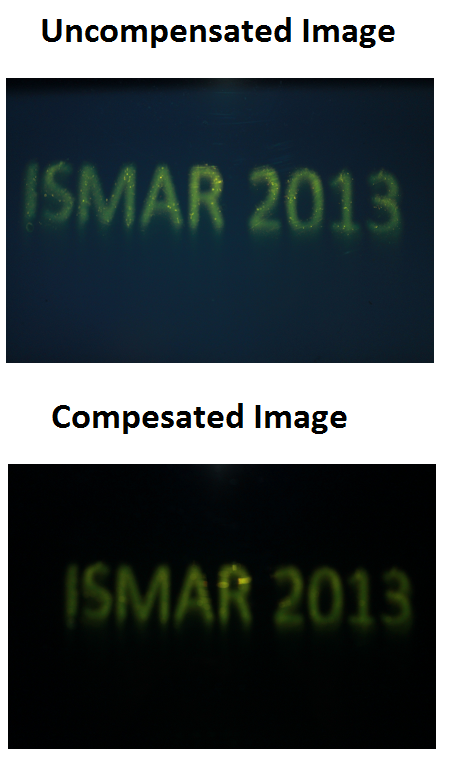
\includegraphics[width=3.0in,height=2.0in]{C:/sri/acmsiggraph/images/example.pdf}
  \caption{Correction results on the p3700 display.}
    \label{fig:Figure14}
\end{figure}

\section{Discussion}
\subsection{Practical Applicability}
Implementing BP-based color correction on additive optical see-through displays requires a display profile and a mechanism to determine how background colors interact with the individual pixels of the display. Ideally, display manufacturers should provide such profile and make it available for developers. In a head-mounted display, the system can use a digital camera for a pixel level mapping of the background and the display image such as in\cite{Bimber:2005}\cite{Weiland:2009}. However, accurate color measurement via a digital camera itself a complex task \cite{Hong:2001}, especially for changing light conditions like the outdoors. A correctly calibrated camera can provide basic background color measurements. For a window-size transparent display such camera-based method is not adequate as it is impossible to locate a camera at the user's vantage point. In such case the system could rely on a 3D model of the background scene with projections of the lighting for a given perspective. Both solutions can support color correction for the \textit{plain} background condition (although the second is less accurate). However, neither of these configurations accounts for the \textit{background} distortion of our model.
\begin{figure}[ht]
  \centering
  \includegraphics[width=2.7in,height=2.0in]{C:/sri/acmsiggraph/images/lvsl.pdf}
  \caption{Effect of the display medium on background L.}
    \label{fig:Figure15}
\end{figure}

To account for the \textit{background} distortion the system should accurately predict how a given background is modified by the display material. A preliminary assessment of 100 colors on the L axis shows the amount of L absorbed by the display material might follow a linear function (see Figure \ref{fig:Figure15}, $R^2$ are almost 1 showing perfect linearity). The effect of the display material on L is significant, particularly for the T-OLED display for which L is reduced by almost half. Further work is required to confirm this trend and to characterize the impact on the hue (A and B).
\subsection{Display Hardware}
We showed an optical see-through display affects color blending through its color profile and its impact on background colors. Limited color profiles such as in the p2200 and T-OLED displays guaranty better BP-based color correction. However, such limited color displays provide a limited color experience for applications like video or game playing. On the other side, full color displays like our p3700 could provide richer color experiences at the cost of less correction accuracy. A promising exploration venue is full color displays with a lower level of transparency. Lower transparency darkens background colors which, as we observed in the correction study in T-OLED display, might be better suited for color correction. The degree of display opacity poses a challenge for how much accessibility and clarity is needed for either the background or the display content, and remains an open question. Ideally, an optical see-through display should provide a way to control the level of transparency at a pixel level, as explored by \cite{Kiyokawa:2003}. A rendering pipeline could rely on BP-based color correction for darker backgrounds and block background light as the correction algorithm approaches its limits (i.e. when high intensity background colors makes the display color uncorrectable).
\subsection{Design Implications}
A major result from our correction study is that, with BP-based color correction, designers can use light neutral colors for information that needs to be preserved best - especially in environments of high luminosity like daytime outdoors. Should more hue be needed, designers can use light colors in the CyanBlue region. Dark colors should be avoided for text and color-encoded information, although they can still be used for creating good contrast (for e.g., text legibility). It is to be noted that the focus of this paper is on preserving digital color on see-through display rather than contrast, which is a design issue.

An important corollary is that even with BP-based color correction, not all display colors can be corrected. The degree by which a display color can be corrected depends to a great extent on the background color. Therefore, interface designers should study the intended normal usage conditions of their application (e.g. outdoors, forest or night time), in order to collect prevalent background colors. Based on such set, designers can analyze how correctable are alternative color palettes on such backgrounds and stick with the one palette which can be corrected the best.
\section{Conclusion}
This paper presents a color correction approach for additive optical see-through displays based on two color distortions introduced by the display: the \textit{render} and \textit{background} distortions. The paper proposes a color blending model that accounts for these two distortions and addresses the \textit{render} distortion by proposing the Binned-Profile (BP) method. The BP method describes the way a particular display renders a representative set of colors of the sRGB gamut. For the second distortion we used colorimetric measurements of how background colors are seen through the display material. We validated the BP-method by measuring the accuracy of its color blend predictions on three different optical see-through displays against other known methods. The results showed that the BP method outperforms other methods, and that this first distortion is the main factor to address for correct color blend predictions.

We presented a color correction algorithm based on the BP-method and investigated its correction capacity using a wide variety of background and display colors for our three displays. Results showed BP-based color correction works best for displays with low color capacity. For displays with high color capacity results show that colors can be better corrected for low intensity backgrounds, and that for high intensity backgrounds light neutrals and CyanBlue colors can be corrected best. We reported our results both graphically (through vertical histograms and heat-maps) and quantitatively.

We finalized with a discussion on the applicability of BP-based color correction including some ideas about addressing the \textit{background} distortion, the impact of display hardware, and implications for interface designers. Our future work includes characterizing the \textit{background} distortion along the lines expressed in the discussion, and testing our approach in the wild with user participants and for different display hardware (i.e. head-mounted displays and window-size transparent displays). We will also explore color blending and correction alternatives for subtractive optical see-through displays such as transparent LCDs.



\section*{Acknowledgements}

NSERC Funding agencie, Lab members in Human computer interaction and University of Manitoba and Saskatchewan.

\bibliographystyle{acmsiggraph}
\bibliography{reference}
\end{document}
